%%%%%%%% ICML 2025 EXAMPLE LATEX SUBMISSION FILE %%%%%%%%%%%%%%%%%

\documentclass{article}

% Recommended, but optional, packages for figures and better typesetting:
\usepackage{microtype}
\usepackage{graphicx}
\usepackage{subfigure}
\usepackage{booktabs} % for professional tables

% hyperref makes hyperlinks in the resulting PDF.
% If your build breaks (sometimes temporarily if a hyperlink spans a page)
% please comment out the following usepackage line and replace
% \usepackage{icml2025} with \usepackage[nohyperref]{icml2025} above.
\usepackage{hyperref}


% Attempt to make hyperref and algorithmic work together better:
\newcommand{\theHalgorithm}{\arabic{algorithm}}

% Use the following line for the initial blind version submitted for review:
% \usepackage{icml2025}

% If accepted, instead use the following line for the camera-ready submission:
\usepackage[accepted]{icml2025}

% For theorems and such
\usepackage{amsmath}
\usepackage{amssymb}
\usepackage{mathtools}
\usepackage{amsthm}

% if you use cleveref..
\usepackage[capitalize,noabbrev]{cleveref}

%%%%%%%%%%%%%%%%%%%%%%%%%%%%%%%%
% THEOREMS
%%%%%%%%%%%%%%%%%%%%%%%%%%%%%%%%
\theoremstyle{plain}
\newtheorem{theorem}{Theorem}[section]
\newtheorem{proposition}[theorem]{Proposition}
\newtheorem{lemma}[theorem]{Lemma}
\newtheorem{corollary}[theorem]{Corollary}
\theoremstyle{definition}
\newtheorem{definition}[theorem]{Definition}
\newtheorem{assumption}[theorem]{Assumption}
\theoremstyle{remark}
\newtheorem{remark}[theorem]{Remark}

% Todonotes is useful during development; simply uncomment the next line
%    and comment out the line below the next line to turn off comments
%\usepackage[disable,textsize=tiny]{todonotes}
\usepackage[textsize=tiny]{todonotes}


% The \icmltitle you define below is probably too long as a header.
% Therefore, a short form for the running title is supplied here:
\icmltitlerunning{Delaunay Rewiring to Avoid Over-Squashing and Over-Smoothing in Graphs}

\begin{document}

\twocolumn[
\icmltitle{Delaunay Rewiring to Avoid Over-Squashing and Over-Smoothing in Graphs}

% It is OKAY to include author information, even for blind
% submissions: the style file will automatically remove it for you
% unless you've provided the [accepted] option to the icml2025
% package.

% List of affiliations: The first argument should be a (short)
% identifier you will use later to specify author affiliations
% Academic affiliations should list Department, University, City, Region, Country
% Industry affiliations should list Company, City, Region, Country

% You can specify symbols, otherwise they are numbered in order.
% Ideally, you should not use this facility. Affiliations will be numbered
% in order of appearance and this is the preferred way.
\icmlsetsymbol{equal}{*}

\begin{icmlauthorlist}
\icmlauthor{Edwin Roussin}{equal,ipp}
\icmlauthor{Tristan Waddington}{equal,ipp}

\end{icmlauthorlist}

\icmlaffiliation{ipp}{Institut Polytechnique de Paris, Palaiseau, France}

\icmlcorrespondingauthor{}{firstname.lastname@polytechnique.edu}

% You may provide any keywords that you
% find helpful for describing your paper; these are used to populate
% the "keywords" metadata in the PDF but will not be shown in the document
\icmlkeywords{Graph, Delaunay, Triangulation, Machine Learning, Over-smoothing, Over-squashing}

\vskip 0.3in
]

% this must go after the closing bracket ] following \twocolumn[ ...

% This command actually creates the footnote in the first column
% listing the affiliations and the copyright notice.
% The command takes one argument, which is text to display at the start of the footnote.
% The \icmlEqualContribution command is standard text for equal contribution.
% Remove it (just {}) if you do not need this facility.

% \printAffiliationsAndNotice{}  % leave blank if no need to mention equal contribution
\printAffiliationsAndNotice{\icmlEqualContribution} % otherwise use the standard text.

\begin{abstract}
This document reviews the graph rewiring method proposed by \cite{attali2024delaunay}[Attali et al, 2024]
based on Delauynay triangulation that aims to avoid over-smoothing and over-squashing
during prediction tasks. It uses notions of edge curvature to measure the quality
of the rewiring. The method is tested on a variety of graph datasets and compared
to another one.
%TODO present other article
\end{abstract}

%%%%%%%%%%%%%%%%%%%%%%%%%%%%%%%%%%%%%%%%%%%%%%%%%%%%%%%%%%%%%%%%%%%%%%%%%%%%%%%
% Delaunay paper
%%%%%%%%%%%%%%%%%%%%%%%%%%%%%%%%%%%%%%%%%%%%%%%%%%%%%%%%%%%%%%%%%%%%%%%%%%%%%%%

\section{Delaunay Rewiring}
\label{delaunay}
Graph neural networks (GNNs) have emerged as the standard approach for effective
learning graph-structured data. GNNs employ an iterative approach, updating node repre-
sentations through the local aggregation of information from
neighboring nodes, known as the message-passing paradigm \cite{gilmer2017neural}.
However, this iterative process can lead to over-smoothing and over-squashing, where
the node representations become too similar to each other, or ineffective to 
transmit long-range information. In these cases, the model performance can degrade.

%%%%%%%%%%%%%%%%%%%%%%%%%%%%%%%%%%%%%%%%%%%%%%%%%%%%%%%%%%%%%%%%%%%%%%%%%%%%%%%
% Theoretical
\subsection{Over-Smoothing and Over-Squashing}

\paragraph{Over-Smoothing}
Message-passing neural networks (MPNN) use an 
iterative approach, updating node representations through 
the local aggregation of information from neighboring nodes.
The need to stack additional layers to capture non-local interactions
tends to make node features more and
more similar, leading to over-smoothing. This is particularly problematic 
when the graph is heterophilic, i.e., when nodes belong to different communities 
\cite{zheng2022graph}.

\paragraph{Over-Squashing}
The squashing effect occurs when the model is unable to transmit
long-range information, leading to a loss of information. MPNN models try to 
capture exponentially growing information into fixed sized representations. 
\cite{alon2021bottleneck} have shown the correlation between overs-quashing and 
 bottleneck in the graph structure.
Models such as Graph Convolutional Networks (GCN) are known to suffer from this issue
because they absorb  the information from all edges equally.

%%%%%%%%%%%%%%%%%%%%%%%%%%%%%%%%%%%%%%%%%%%%%%%%%%%%%%%%%%%%%%%%%%%%%%%%%%%%%%%
\subsection{Edge Curvature}
The main metrics used to characterize graph structure and measure the quality
of the rewiring is the discrete Ricci edge curvature. A complete definition can be found on 
\cref{app:curvature}. Previous work has shown that:
\begin{itemize}
    \item Positive curvature edges establish connections between 
        nodes belonging to the same community.
        Highly positive curved edges cause over-smoothing \cite{nguyen2023revisiting}.
                
    \item Negative curvature edges connect nodes from different communities.
        Highly negative curved edges cause over-squashing \cite{topping2022understandingoversquashingbottlenecksgraphs}.
\end{itemize}
\begin{figure}[ht]
    \label{fig:edge_curvature}
    \vskip -0.2in
    \begin{center}
    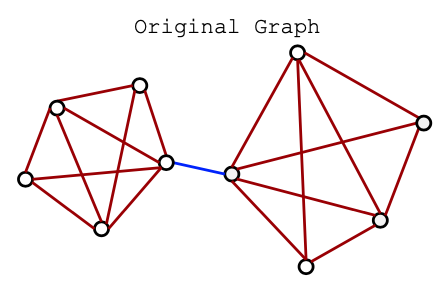
\includegraphics[width=0.6\columnwidth]{figures/original_graph.png}
    \caption{\scriptsize Example graph: in red the edges with positive curvature ($\sim 3$), 
    in blue with negative curvature (-1.2) \cite{attali2024delaunay}}
    \end{center}
    \vskip -0.2in
\end{figure}
\textbf{Hence, we get a simple metric for further experiments where we expect to see the 
edge curvature amplitude decrease after the rewiring process.}

%%%%%%%%%%%%%%%%%%%%%%%%%%%%%%%%%%%%%%%%%%%%%%%%%%%%%%%%%%%%%%%%%%%%%%%%%%%%%%%
\subsection{Rewiring}
\subsubsection{Former methods' limitation}
Existing methods mitigate over-squashing by rewiring
the input graph to minimize structural bottlenecks. 
First ones rely on the analysis of the graph structure, through local or global features
like edge curvature or resistance. However, these methods may not scale well with 
the number of nodes and need depends on the choice of hyperparameters. 
Moreovoer, they modify the original graph, which is not always available in some applications.

Conversely, over-smoothing is avoided by preventing embedding to become the same 
through: \textbf{Normalization} with PairNorm \cite{zhao2020pairnorm}; 
or \textbf{rewiring} dropping edges, at random \cite{rong2019dropedge} 
or in finding the potential good ones \cite{Giraldo_2023}

\subsubsection{Delaunay Triangulation}
\paragraph{Delaunay rewiring}
Is an extreme \textbf{4 steps rewiring} method illustrated bellow.
\begin{enumerate}
    \item A first GNN\footnote{GCN from \cite{kipf2017semi}} constructs 
        \textbf{node embeddings} from the original graph.
    \item Reduce the embedding with \textbf{UMAP} in dim 2.
    \item \textbf{Rebuilt edges with Delaunay triangulation} from their distance in UMAP embedding space.
    \item Second GNN \textbf{mix} the Delaunay graph with the original features 
    from the beginning.
\end{enumerate}
\begin{figure}[ht!]
    \begin{center}
    \label{fig:delaunay_rewiring}
    \vskip -0.2in
    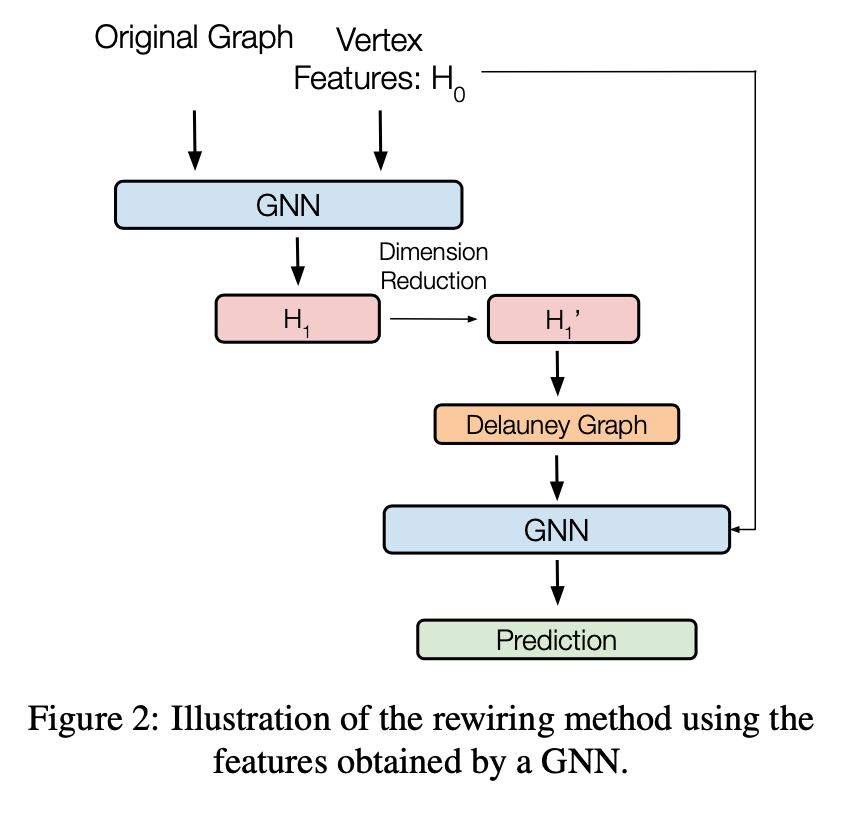
\includegraphics[width=0.9\columnwidth]{figures/Rewiring_method.png}
    %\caption{Illustration of the Delaunay [Attali al., 2024] \cite{attali2024delaunay}}
    \vskip -0.2in
    \end{center}
    \end{figure}

\paragraph{Initial throughts}
The method is remarkably simple, as it does not require any hyperparameters according to authors, 
which eliminates the need for a grid search. Its computational complexity is 
efficient, scaling as $\mathcal{O} \big( N \log N \big)$. 
Additionally, the method constructs a graph directly from the embedding, 
making it independent of the presence of the original graph.

The use of UMAP is restricted to two dimensions. This is because performing 
triangulation in higher dimensions increases computation time and 
results in denser graphs\footnote{Generalized triangles in three dimensions
 have six edges, while in four dimensions, they have ten edges.}. 
This increased density reduced the accuracy in experiments, making the two-dimensional approach more practical and effective.

Authors have added the first GNN late in their research as the Delaunay Graph 
need quality embedding. However, it raises questions about whether these initial
representation are victims of smoothing and squashing effects by this GNN.
Does this GNN effectively captures long-range dependencies?


%%%%%%%%%%%%%%%%%%%%%%%%%%%%%%%%%%%%%%%%%%%%%%%%%%%%%%%%%%%%%%%%%%%%%%%%%%%%%%%
\subsection{Experiments}
We habve reproduce the rewiring experiment on the \textbf{Wisconsin dataset}\footnote{
From WebKB dataset, 251 nodes = web pages from Wisconsin connected
by edges = hyperlinks, node features = bag-of-words in dim 1703, labels =  5 kind of author.}.
This report presents a comprehensive evaluation of the Delaunay rewiring 
approach, demonstrating substantial improvements in graph neural network performance:

\textbf{Key Results}:
\begin{itemize}
    \item GCN accuracy improved from 54.90\% to 67.55\% (+12.6\%)
    \item GAT accuracy improved from 55.88\% to 69.12\% (+13.2\%)
    \item Graph homophily increased by 96\% (0.366 $\to$ 0.718)
    \item All improvements are statistically significant ($p < 0.0001$)
\end{itemize}

\begin{table}[h!]
\caption{Comparison of Baseline and Delaunay Graph Metrics}
\centering
\begin{tabular}{|l|c|c|}
\hline
\textbf{Metric}          & \textbf{Orignal} & \textbf{Delaunay Graph} \\ \hline
Mean Degree              & 5.59                   & 7.85               \\ \hline
Homophily                & 0.366                  & 0.710 ($\uparrow$ 96\%) \\ \hline
Curvature Range          & [-0.475, 0.250]        & [-0.214, 0.200]         \\ \hline
\end{tabular}



\label{tab:graph_comparison}
\end{table}
    
\textbf{Impact}: The Delaunay rewiring approach successfully addresses 
over-squashing and improves graph structure, leading to significant performance 
gains across different model architectures.

\textbf{Validation}: Results are robust across multiple experiments and 
statistically significant, with comprehensive analysis of graph properties
supporting the improvements.

%%%%%%%%%%%%%%%%%%%%%%%%%%%%%%%%%%%%%%%%%%%%%%%%%%%%%%%%%%%%%%%%%%%%%%%%%%%%%%%
\subsection{Limitations}
\paragraph{Dimensionality Reduction} We might lose some feature information
during the UMAP reduction to 2 dimensions. The quality of Delaunay graph depends
 on quality of reduced features.

 \paragraph{Computational Considerations}
 The method complexity is in $\mathcal{O} \big( N \log N \big)$ only, but the 
 two graphs are  fully loaded into memory. Furthermore, the UMAP and curvature 
 computation can cause overhead, but this is way better than the quadratic cost
 of other methods.
   
\paragraph{Parameter Sensitivity} We do not totally agree with the authors as
we find out that the impact of UMAP parameters not fully explored. They could
modulate the quality of the embedding we already discussed. Moreover, the
potential dependence on feature normalization and the effect of different
 train/val/test splits is not extensively studied.

\subsection{Future Work}
If we were to work further in this topic, we could focus on:
\begin{itemize}
    \item \textbf{Algorithmic Improvements}: Investigate higher-dimensional 
    Delaunay triangulation, explore sparse approximations for larger graphs, 
   Develop incremental/streaming versions for large-scale graphs or 
   optimize UMAP parameter selection.

    \item \textbf{Analysis Extensions}:
   Study impact on different graph properties, 
   investigate relationship between feature space and graph structure,
   compare with other rewiring methods on the same dataset,
   or analyze feature importance in graph construction.

    \item \textbf{Ablation Studies}:
   Compare with other dimensionality reduction method, the effect of different 
   feature preprocessing, the sensitivity to hyperparameters and try different
    triangulation algorithms.
\end{itemize}

%%%%%%%%%%%%%%%%%%%%%%%%%%%%%%%%%%%%%%%%%%%%%%%%%%%%%%%%%%%%%%%%%%%%%%%%%%%%%%%
% Other paper
%%%%%%%%%%%%%%%%%%%%%%%%%%%%%%%%%%%%%%%%%%%%%%%%%%%%%%%%%%%%%%%%%%%%%%%%%%%%%%%
\section{Additional Paper}

% TODO
%%%%%%%%%%%%%%%%%%%%%%%%%%%%%%%%%%%%%%%%%%%%%%%%%%%%%%%%%%%%%%%%%%%%%%%%%%%%%%%
\subsection{Choice explanation}

%%%%%%%%%%%%%%%%%%%%%%%%%%%%%%%%%%%%%%%%%%%%%%%%%%%%%%%%%%%%%%%%%%%%%%%%%%%%%%%
\subsection{Paper summary}

%%%%%%%%%%%%%%%%%%%%%%%%%%%%%%%%%%%%%%%%%%%%%%%%%%%%%%%%%%%%%%%%%%%%%%%%%%%%%%%
\subsection{Comparison}






%%%%%%%%%%%%%%%%%%%%%%%%%%%%%%%%%%%%%%%%%%%%%%%%%%%%%%%%%%%%%%%%%%%%%%%%%%%%%%%
% Template conclusion
%%%%%%%%%%%%%%%%%%%%%%%%%%%%%%%%%%%%%%%%%%%%%%%%%%%%%%%%%%%%%%%%%%%%%%%%%%%%%%%

\section*{Software and Data}

The original code repository and additional work can be found on GitHub\footnote{ 
\url{https://github.com/waddason/Delaunay-Rewiring}}.
The code is written in Python and uses the PyTorch library. The code is available under the MIT license.

% Acknowledgements should only appear in the accepted version.
\section*{Acknowledgements}

We thank our professor Mr. Jhony H. Giraldo for presenting us this article and 
the theoretical foundations to understand it.

\section*{Impact Statement}

This paper highlight the promising yet simple method of Delauynay Rewirin to 
improve the performance of graph-based machine learning models.
We hope to see this method adopted.


% In the unusual situation where you want a paper to appear in the
% references without citing it in the main text, use \nocite
% \nocite{langley00}

\bibliography{references}
\bibliographystyle{icml2025}


%%%%%%%%%%%%%%%%%%%%%%%%%%%%%%%%%%%%%%%%%%%%%%%%%%%%%%%%%%%%%%%%%%%%%%%%%%%%%%%
%%%%%%%%%%%%%%%%%%%%%%%%%%%%%%%%%%%%%%%%%%%%%%%%%%%%%%%%%%%%%%%%%%%%%%%%%%%%%%%
% APPENDIX
%%%%%%%%%%%%%%%%%%%%%%%%%%%%%%%%%%%%%%%%%%%%%%%%%%%%%%%%%%%%%%%%%%%%%%%%%%%%%%%
%%%%%%%%%%%%%%%%%%%%%%%%%%%%%%%%%%%%%%%%%%%%%%%%%%%%%%%%%%%%%%%%%%%%%%%%%%%%%%%
\newpage
\appendix
\onecolumn

\section{Additional details on the Delaunay Rewiring }
\label{app:delaunay}
\begin{figure}[h!]
    \label{fig:delaunay_full}
    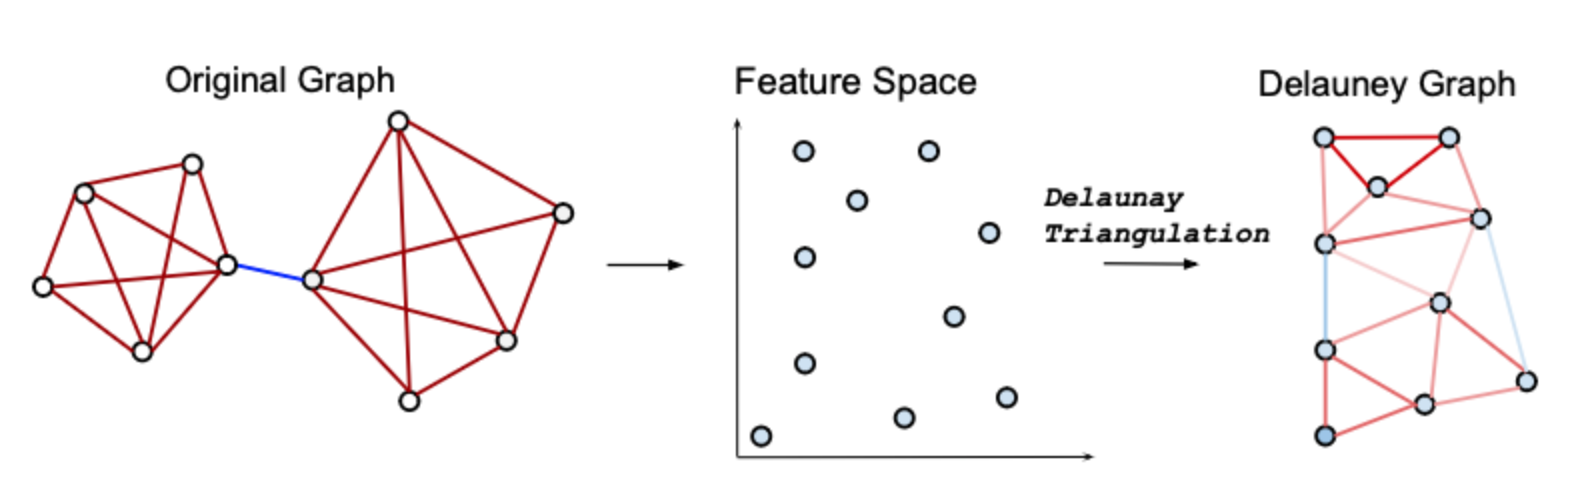
\includegraphics[width=0.9\textwidth]{figures/delaunay_process.png}
    \caption{Illustration of the Delaynay rewiring process in a 2-dimension feature space.}
\end{figure}

\section{Edge Curvature}
\label{app:curvature}

Paper: Balance Forman Curvature \cite{topping2022understandingoversquashingbottlenecksgraphs} is computed over cycles of size 4.\\
    \emph{Experiment: Oliver-Ricci Curvature \cite{ni2015riccicurvatureinternettopology}} {\scriptsize
    \texttt{GraphRicciCurvature.OllivierRicci}.
    }\\
    $$c_{ij}= \frac{2}{d_i} + \frac{2}{d_j} - 2 + 2 \frac{\sharp_{\Delta}}{\max(d_i, d_j)} + 
            \frac{\sharp_{\Delta}}{\min(d_i, d_j)} + 
            \frac{\max(\sharp_{\square}^i,\sharp_{\square}^j)^{-1}}{\max(d_i, d_j)}
            (\sharp_{\square}^i + \sharp_{\square}^j)
    $$

    where $\sharp_{\Delta}$ is the number of triangles based at $e_{ij}$, 
    $\sharp_{\square}^i$ is the number of 4-cycles based at $e_{ij}$ starting from $i$
    without diagonals inside.


    
%%% EXAMPLES
\begin{figure}[ht]
    \vskip 0.2in
    \begin{center}
    \centerline{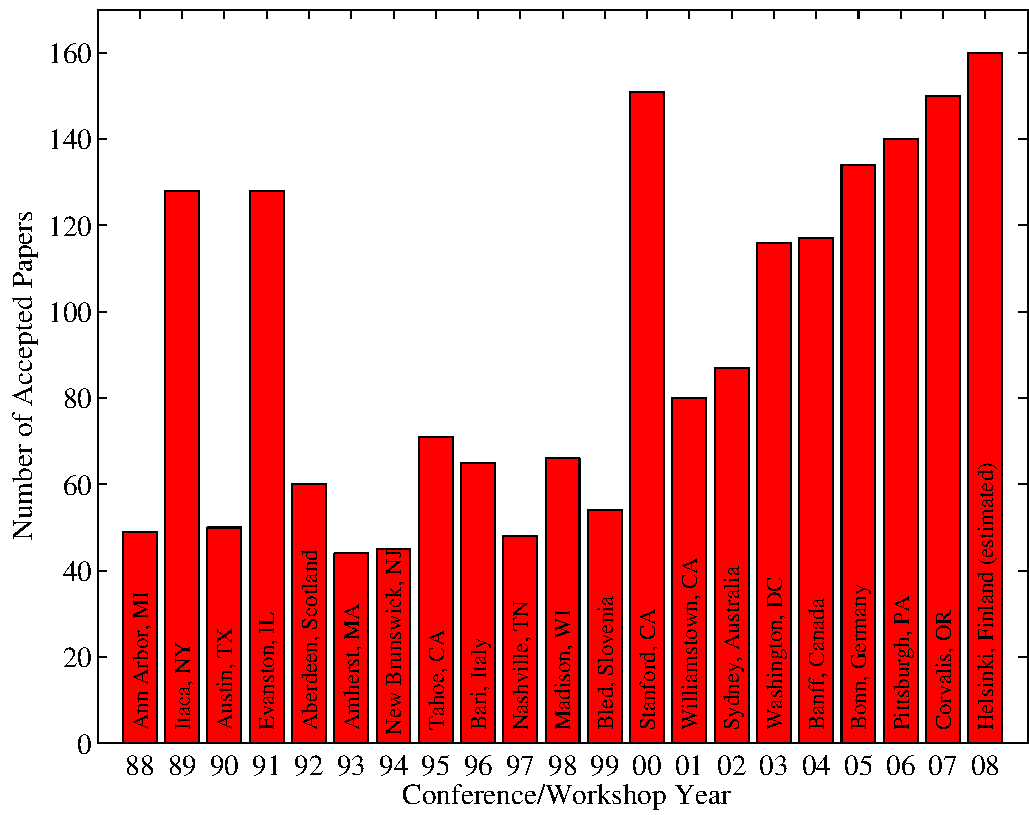
\includegraphics[width=\columnwidth]{icml_numpapers}}
    \caption{Historical locations and number of accepted papers for International
    Machine Learning Conferences (ICML 1993 -- ICML 2008) and International
    Workshops on Machine Learning (ML 1988 -- ML 1992). At the time this figure was
    produced, the number of accepted papers for ICML 2008 was unknown and instead
    estimated.}
    \label{icml-historical}
    \end{center}
    \vskip -0.2in
    \end{figure}
    
    \subsection{Figures}
    
    You may want to include figures in the paper to illustrate
    your approach and results. Such artwork should be centered,
    legible, and separated from the text. Lines should be dark and at
    least 0.5~points thick for purposes of reproduction, and text should
    not appear on a gray background.
    
    Label all distinct components of each figure. If the figure takes the
    form of a graph, then give a name for each axis and include a legend
    that briefly describes each curve. Do not include a title inside the
    figure; instead, the caption should serve this function.
    
    Number figures sequentially, placing the figure number and caption
    \emph{after} the graphics, with at least 0.1~inches of space before
    the caption and 0.1~inches after it, as in
    \cref{icml-historical}. The figure caption should be set in
    9~point type and centered unless it runs two or more lines, in which
    case it should be flush left. You may float figures to the top or
    bottom of a column, and you may set wide figures across both columns
    (use the environment \texttt{figure*} in \LaTeX). Always place
    two-column figures at the top or bottom of the page.
    
    \subsection{Algorithms}
    
    If you are using \LaTeX, please use the ``algorithm'' and ``algorithmic''
    environments to format pseudocode. These require
    the corresponding stylefiles, algorithm.sty and
    algorithmic.sty, which are supplied with this package.
    \cref{alg:example} shows an example.
    
    \begin{algorithm}[tb]
       \caption{Bubble Sort}
       \label{alg:example}
    \begin{algorithmic}
       \STATE {\bfseries Input:} data $x_i$, size $m$
       \REPEAT
       \STATE Initialize $noChange = true$.
       \FOR{$i=1$ {\bfseries to} $m-1$}
       \IF{$x_i > x_{i+1}$}
       \STATE Swap $x_i$ and $x_{i+1}$
       \STATE $noChange = false$
       \ENDIF
       \ENDFOR
       \UNTIL{$noChange$ is $true$}
    \end{algorithmic}
    \end{algorithm}
    
    \subsection{Tables}
    
    You may also want to include tables that summarize material. Like
    figures, these should be centered, legible, and numbered consecutively.
    However, place the title \emph{above} the table with at least
    0.1~inches of space before the title and the same after it, as in
    \cref{sample-table}. The table title should be set in 9~point
    type and centered unless it runs two or more lines, in which case it
    should be flush left.
    
    % Note use of \abovespace and \belowspace to get reasonable spacing
    % above and below tabular lines.
    
    \begin{table}[t]
    \caption{Classification accuracies for naive Bayes and flexible
    Bayes on various data sets.}
    \label{sample-table}
    \vskip 0.15in
    \begin{center}
    \begin{small}
    \begin{sc}
    \begin{tabular}{lcccr}
    \toprule
    Data set & Naive & Flexible & Better? \\
    \midrule
    Breast    & 95.9$\pm$ 0.2& 96.7$\pm$ 0.2& $\surd$ \\
    Cleveland & 83.3$\pm$ 0.6& 80.0$\pm$ 0.6& $\times$\\
    Glass2    & 61.9$\pm$ 1.4& 83.8$\pm$ 0.7& $\surd$ \\
    Credit    & 74.8$\pm$ 0.5& 78.3$\pm$ 0.6&         \\
    Horse     & 73.3$\pm$ 0.9& 69.7$\pm$ 1.0& $\times$\\
    Meta      & 67.1$\pm$ 0.6& 76.5$\pm$ 0.5& $\surd$ \\
    Pima      & 75.1$\pm$ 0.6& 73.9$\pm$ 0.5&         \\
    Vehicle   & 44.9$\pm$ 0.6& 61.5$\pm$ 0.4& $\surd$ \\
    \bottomrule
    \end{tabular}
    \end{sc}
    \end{small}
    \end{center}
    \vskip -0.1in
    \end{table}
    
    Tables contain textual material, whereas figures contain graphical material.
    Specify the contents of each row and column in the table's topmost
    row. Again, you may float tables to a column's top or bottom, and set
    wide tables across both columns. Place two-column tables at the
    top or bottom of the page.
    
    \subsection{Theorems and such}
    The preferred way is to number definitions, propositions, lemmas, etc. consecutively, within sections, as shown below.
    \begin{definition}
    \label{def:inj}
    A function $f:X \to Y$ is injective if for any $x,y\in X$ different, $f(x)\ne f(y)$.
    \end{definition}
    Using \cref{def:inj} we immediate get the following result:
    \begin{proposition}
    If $f$ is injective mapping a set $X$ to another set $Y$, 
    the cardinality of $Y$ is at least as large as that of $X$
    \end{proposition}
    \begin{proof} 
    Left as an exercise to the reader. 
    \end{proof}
    \cref{lem:usefullemma} stated next will prove to be useful.
    \begin{lemma}
    \label{lem:usefullemma}
    For any $f:X \to Y$ and $g:Y\to Z$ injective functions, $f \circ g$ is injective.
    \end{lemma}
    \begin{theorem}
    \label{thm:bigtheorem}
    If $f:X\to Y$ is bijective, the cardinality of $X$ and $Y$ are the same.
    \end{theorem}
    An easy corollary of \cref{thm:bigtheorem} is the following:
    \begin{corollary}
    If $f:X\to Y$ is bijective, 
    the cardinality of $X$ is at least as large as that of $Y$.
    \end{corollary}
    \begin{assumption}
    The set $X$ is finite.
    \label{ass:xfinite}
    \end{assumption}
    \begin{remark}
    According to some, it is only the finite case (cf. \cref{ass:xfinite}) that is interesting.
    \end{remark}
    %restatable


%%%%%%%%%%%%%%%%%%%%%%%%%%%%%%%%%%%%%%%%%%%%%%%%%%%%%%%%%%%%%%%%%%%%%%%%%%%%%%%
%%%%%%%%%%%%%%%%%%%%%%%%%%%%%%%%%%%%%%%%%%%%%%%%%%%%%%%%%%%%%%%%%%%%%%%%%%%%%%%


\end{document}


% This document was modified from the file originally made available by
% Pat Langley and Andrea Danyluk for ICML-2K. This version was created
% by Iain Murray in 2018, and modified by Alexandre Bouchard in
% 2019 and 2021 and by Csaba Szepesvari, Gang Niu and Sivan Sabato in 2022.
% Modified again in 2023 and 2024 by Sivan Sabato and Jonathan Scarlett.
% Previous contributors include Dan Roy, Lise Getoor and Tobias
% Scheffer, which was slightly modified from the 2010 version by
% Thorsten Joachims & Johannes Fuernkranz, slightly modified from the
% 2009 version by Kiri Wagstaff and Sam Roweis's 2008 version, which is
% slightly modified from Prasad Tadepalli's 2007 version which is a
% lightly changed version of the previous year's version by Andrew
% Moore, which was in turn edited from those of Kristian Kersting and
% Codrina Lauth. Alex Smola contributed to the algorithmic style files.
